\section{Konfigurationsmanagement}
Beim Konfigurationsmanagement handelt es sich um die Entwicklung und Anwendung von Standards und Verfahren zur Verwaltung eines sich weiterentwickelnden Systemprodukts.
\subsection{Einleitung}
\subsubsection{Fragestellungen}
\begin{itemize}
	\item Das System lief gestern noch; was hat sich seitdem geändert?
	\item Wer hat diese (fehlerhafte?) Änderung wann und warum durchgeführt?
	\item Wer ist von meinen Änderungen an dieser Datei betroffen?
	\item Auf welche Version des Systems bezieht sich die Fehlermeldung?
	\item Wie erzeuge ich Version x.y aus dem Jahre 1999 wieder?
	\item Welche Fehlermeldungen sind in dieser Version bereits bearbeitet?
	\item Welche Erweiterungswünsche liegen für das nächste Release vor?
	\item  Die Platte ist hinüber; was für einen Status haben die Backups?
\end{itemize}
\subsubsection{Definitionen}
\paragraph{Definition von Software-KM nach IEEE-Standard 828-1988}
SCM (Software Configuration Management) constitutes \textbf{good engineering practice } for all software projects, whether phased development, rapid prototyping, or ongoing  maintenance. It enhances the reliability and quality of software by:
\begin{itemize}
	\item Providing structure for \textbf{identifying and controlling} documentation, code, interfaces, and databases to support all life cycle phases
	\item Supporting a chosen \textbf{development/maintenance methodology} that fits the requirements, standards, policies, organization, and management philosophy
	\item Producing \textbf{management and product information} concerning the status of baselines, change control, tests, releases, audits etc.
\end{itemize}
Diese Definition ist jedoch nicht konkret und unabhängig vom Begriff ''Software''
\paragraph{Definition nach DIN EN ISO 10007}
KM (Konfigurationsmanagement) ist eine Managementdisziplin, die über die gesamte Entwicklungszeit eines Erzeugnisses angewandt wird, um Transparenz und Überwachung seiner funktionellen und physischen Merkmale sicherzustellen.
\\
Der KM-Prozess umfasst die folgenden integrierten Tätigkeiten:
\begin{itemize}
	\item \textbf{Konfigurationsidentifizierung}: Definition und Dokumentation der Bestandteile eines Erzeugnisses, Einrichten von Bezugskonfigurationen, ...
	\item \textbf{Konfigurationsüberwachung}: Dokumentation und Begründung von Änderungen, Genehmigung oder Ablehnung von Änderungen, Planung von Freigaben, ...
	\item \textbf{Konfigurationsbuchführung}: Rückverfolgung aller Änderungen bis zur letzten Bezugskonfiguration, ...
	\item \textbf{Konfigurationsauditierung}: Qualitätssicherungsmaßnahmen für Freigabe einer Konfiguration eines Erzeugnisses
	\item \textbf{KM-Planung}: Festlegung der Grundsätze und Verfahren zum KM in Form eines KM-Plans
\end{itemize}
\paragraph{Werkzeugorientierte Sicht auf KM-Aktivitäten}
\begin{enumerate}
	\item \textbf{KM-Planung}: Beschreibung der Standards, Verfahren und Werkzeuge, die für KM benutzt werden; wer darf/muss wann was machen
	\item \textbf{Versionsmanagement}: Verwaltung der Entwicklungsgeschichte eines Produkts; also wer hat wann, wo, was und warum geändert
	\item \textbf{Variantenmanagement}: Verwaltung parallel existierender Ausprägungen eines Produkts für verschiedene Anforderungen, Länder, Plattformen
	\item \textbf{Releasemanagement}: Verwaltung und Planung von Auslieferungsständen; wann wird eine neue Produktversion mit welchen Features auf den Markt geworfen  
	\item \textbf{Buildmanagement}: Erzeugung des auszulieferenden Produkts; wann muss welche Datei mit welchem Werkzeug generiert, übersetzt, ... werden
	\item \textbf{Änderungsmanagement}: Verwaltung von Änderungsanforderungen; also Bearbeitung von Fehlermeldungen und Änderungswünschen (Feature Requests) sowie Zuordnung zu Auslieferungsständen
\end{enumerate}
\begin{figure}[h]
	\caption{Integration des Konfigurationsmanagements im V-Modell}
	\centering
	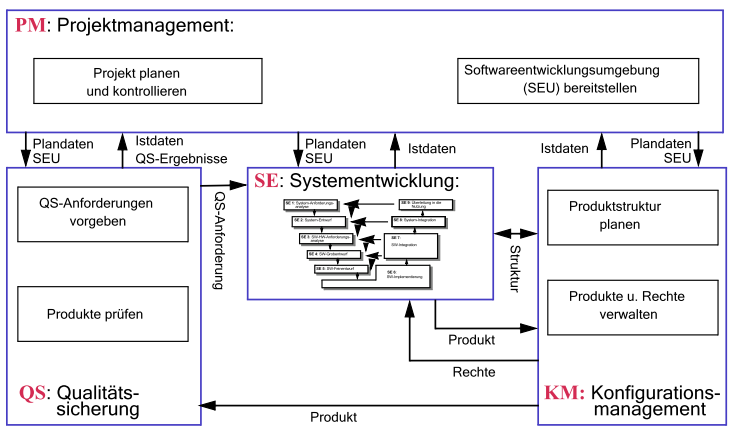
\includegraphics[width=0.85\textwidth]{2_1_1}
\end{figure}
\begin{figure}[h]
	\caption{Grafische Übersicht über Aufgaben- und Rollenverteilung}
	\centering
	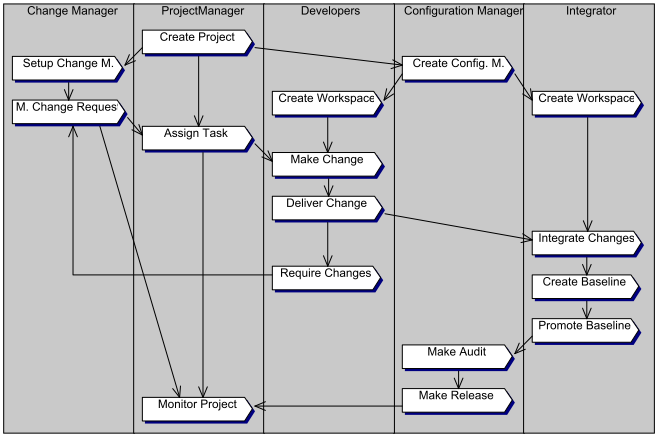
\includegraphics[width=0.85\textwidth]{2_1_2}
\end{figure}
\paragraph{Workspaces für das Konfigurationsmanagement}
\begin{figure}[h]
	\caption{Workspaces für das Konfigurationsmanagement}
	\centering
	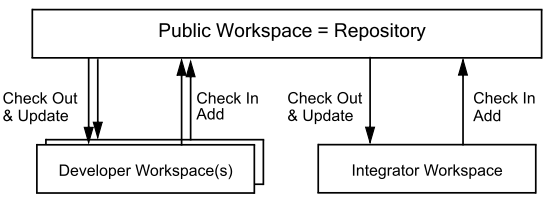
\includegraphics[width=0.6\textwidth]{2_1_3}
\end{figure}
\begin{itemize}
	\item alle Dokumente (Objekte, Komponenten) zu einem bestimmten Projekt werden in	einem gemeinsamen Repository (\textbf{public workspace}) aufgehoben
	\item im Repository werden nicht nur aktuelle Versionen, sondern auch alle \textbf{früheren Versionen} aller Dokumenten gehalten
	\item beteiligte Entwickler bearbeiten ihre eigenen Versionen dieser Dokumente in 
	ihrem privaten Arbeitsbereich (private workspace, \textbf{developer workspace}) 
	\item es gibt genau einen Integrationsarbeitsbereich (\textbf{integrations workspace}) für die Systemintegration
\end{itemize}
\paragraph{Aktivitäten bei der Arbeit mit Workspaces}
\begin{itemize}
	\item Personen holen sich Versionen neuer Dokumente, die von anderen Personen erstellt wurden(\textbf{checkout}), ih ihren privaten Arbeitsbereich
	\item Personen passen ihre Privatversionen ggf. von Zeit zu Zeit an neue Versionen im öffentlichen Repository an (\textbf{update}).
	\item Sie fügen (hoffentlich) nur konsistente Dokumente als neue Versionen in das allgemeine Repository ein (\textbf{checkin = commit}).
	\item Ab und an werden neue Dokumente dem Repository hinzugefügt (\textbf{add}). 
	\item Jede Person kann alte/neue Versionen frei wählen.
\end{itemize}
\paragraph{Probleme}
\begin{itemize}
	\item Wie wird Konsistenz von Gruppen abhängiger Dokumente sichergestellt?
	\item Was passiert bei gleichzeitigen Änderungswünschen für ein Dokument?
	\item Wie realisiert man die Repository-Operationen effizient?
	\item Wie unterstützt man ''Offline''-Arbeit (ohne Zugriff auf Repository)?
\end{itemize}
\paragraph{Weitere Begriffe des Konfigurationsmanagements}
\begin{itemize}
	\item \textbf{Dokument} = Gegenstand, der der Konfigurationsverwaltung unterworfen wird (eine einzelne Datei oder ein ganzer Dateibaum oder ... )
	\item \textbf{(Versions-)Objekt} = Zustand einer Dokument zu einem bestimmten Zeitpunkt in einer bestimmten Ausprägung
	\item \textbf{Varianten} = parallel zueinander (gleichzeitig) existierende Ausprägungen eines Dokuments, die unterschiedliche Anforderungen erfüllen
	\item \textbf{Revisionen} = zeitlich aufeinander folgende Zustände eines Dokuments
	\item  \textbf{Konfiguration} = komplexes Versionsobjekt, eine bestimmte Ausprägung eines Programmsystems (oft hierarchisch strukturierte Menge von Dokumenten)
	\item \textbf{Baseline} = eine Konfiguration, die zu einem Meilenstein (Ende einer Entwicklungsphase) gehört und evaluiert (getestet) wird
	\item \textbf{Release} = eine stabile Baseline, die ausgeliefert wird (intern an Entwickler oder extern an bestimmte Kunden oder ... )
\end{itemize}
\subsection{Versionsmanagement}
Bekannteste ''open source''-Produkte (in zeitlicher Reihenfolge) sind:
\begin{itemize}
	\item Source Code Control System \textbf{SCCS} von AT\&T (Bell Labs):
	\begin{itemize}
		\item effiziente Speicherung von Textdateiversionen als ''Patches''
	\end{itemize}
	\item Revision Control System \textbf{RCS} von Berkley/Purdue University
	\begin{itemize}
		\item schnellerer Zugriff auf Textdateiversionen
	\end{itemize}
	\item Concurrent Version (Control) System \textbf{CVS} (zunächst Skripte für RCS)
	\begin{itemize}
		\item Verwaltung von Dateibäumen
		\item parallele Bearbeitung von Textdateiversionen
	\end{itemize}
	\item Subversion \textbf{SVN} - CVS-Nachfolger von CollabNet initiiert (http://www.collab.net)
	\begin{itemize}
		\item Versionierung von Dateibäumen
	\end{itemize}
	\item \textbf{Git}, Mercurial, ... als verteilte Versionsmanagementsysteme
	\begin{itemize}
		\item jeder Entwickler hat eigene/lokale Versionsverwaltung
	\end{itemize}
\end{itemize}
\subsubsection{Source Code Control System SCCS von AT\&T (Bell Labs)}
Je Dokument (Quelltextdatei) gibt es eine eigene \textbf{History-Datei}, die alle Revisionen als eine Liste jeweils geänderter (Text-)Blöcke speichert:
\begin{itemize}
	\item jeder Block ist ein \textbf{Delta}, das Änderungen zwischen Vorgängerrevision und aktueller Revision beschreibt
	\item jedes Delta hat \textbf{SCCS-Identifikationsnummer} der zugehörigen Revision: <ReleaseNo>.<LevelNo>.<BranchNo>.<SequenceNo>
\end{itemize}
\paragraph{Revisionsbäume von SCSS}
\begin{itemize}
	\item Release 1.1 \ Neuentwicklung
	\item Release 1.1 \ Wartung
	\item Release 1.2 \ Weiterentwicklung
	\item Release 2 \ Weiterentwicklung
\end{itemize}
\paragraph{Erläuterungen zu ''diff'' und ''patch''}
\begin{itemize}
	\item ''\textbf{diff}''-Werkzeug bestimmt Unterschiede zwischen (Text-)Dateien = \textbf{Deltas}
	\item ein Delta(diff) zwischen zwei Textdateien besteht aus einer Folge von ''Hunks'', die jeweils Änderungen eines Zeilenbereichs beschreiben:
	\begin{itemize}
		\item Änderungen von Zeilen: werden mit ''\textbf{!}'' markiert
		\item Hinzufügen von Zeilen: werden mit ''\textbf{+}'' markiert
		\item Löschen von Zeilen: werden mit ''\textbf{-}'' markiert
	\end{itemize}
	\item reale Deltas enthalten unveränderte \textbf{Kontextzeilen} zur besseren Identifikation von Änderungsstellen
	\item ein \textbf{Vorwärtsdelta} zwischen zwei Dateien d1 und d2 kann als ''\textbf{patch}'' zur Erzeugung von Datei d2 auf Datei d1 angewendet werden
	\item inverses \textbf{Rückwärtsdelta} zwischen zwei Dateien d1 und d2 kann als ''patch'' zur Wiederherstellung von Datei d1 auf Datei d2 angewendet werden
	\item SCCS-Deltas sind in einer Datei gespeichert, deshalb weder Vorwärts- noch Rückwärts- sondern \textbf{Inline-Deltas}
\end{itemize}
\paragraph{Genauere Instruktionen zur Erzeugung von Deltas}
Jedes ''diff''-Werkzeug hat seine eigenen Heuristiken, wie es möglichst kleine und/oder lesbare Deltas/Patches erzeugt, die die Unterschiede zweier Dateien darstellen. Ein möglicher (und in den Übungen verwendeter) Satz von Regeln zur Erzeugung von Deltas sieht wie folgt aus:
\begin{enumerate}
	\item Die Anzahl der geänderten, gelöschten und neu erzeugten Zeilen aller Hunks eines \textbf{Deltas} zweier Dateien wird möglichst klein gehalten.
	\item Jeder Hunk beginnt mit genau einer unveränderten \textbf{Kontextzeile} und enthält sonst nur geänderte, gelöschte oder neu eingefügte Zeilen (Ausnahme: Dateianfang).
	\item Aufeinander folgende Hunks sind also durch jeweils \textbf{mindestens eine unveränderte Zeile} getrennt.
	\item Optional: Anstelle von Löschen und Neuerzeugen einer Zeile i verwendet man die 
	\textbf{Änderungsmarkierung ''!''}
\end{enumerate}
\paragraph{Durch diese Regeln nicht gelöstes Problem}
Wie erkenne ich, ob eine Änderung in Zeile i durch Einfügen einer neuen Zeile oder durch Ändern einer alten Zeile zustande gekommen ist?
\paragraph{Create- und Apply-Patch in Eclipse}
Die ''Create Patch''- und ''Apply Patch''-Funktionen in Eclipse benutzen genau das gerade eingeführte ''Unified Diff''-Format. Dabei werden bei der Erzeugung von Hunks wohl folgende Heuristiken/Regeln verwendet:
\begin{itemize}
	\item ein Hunk scheint in der Regel mit drei unveränderten Kontextzeilen zu beginnen (inklusive Leerzeilen).
	\item zwei Blöcke geänderter Zeilen müssen durch mindestens sieben unveränderte Zeilen getrennt sein, damit dafür getrennte Hunks erzeugt werden
\end{itemize}
Bei der Anwendung von Patches werden folgende Heuristiken/Regeln verwendet:
\begin{itemize}
	\item werden der Kontext oder die zu löschenden Zeilen eines Patches so nicht gefunden, dann endet die Patch-Anwendung mit einer Fehlermeldung
	\item befindet sich die zu patchende Stelle eines Textes nicht mehr an der angegebenen Stelle (Zeile), so wird trotzdem der Patch angewendet
	\item gibt es mehrere (identische) Stellen in einem Text, auf die ein Patch angewendet werden kann, so wird die Stelle verändert, die am nächsten zur alten Position ist
\end{itemize}
\paragraph{Eigenschaften von SCSS}
\begin{itemize}
	\item für beliebinge (Text-)Dateien verwendbar (und nur für solche
	\item Schreibsperren auf ''ausgecheckten'' Revisionen
	\item Revisionsbäume mit manuellem Konsistenthalten von Entwicklungszweigen
	\item Rekonstruktionszeit von Revisionen steigt linear mit der Anzahl der Revisionen (Durchlauf durch Blockliste)
	\item Revisionsidentifikation nur durch Nummer und Datum
\end{itemize}
\paragraph{Offene Probleme}
\begin{itemize}
	\item Kein Konfigurationsbegriff und kein Variantenbegriff
	\item Keine Unterstützung zur Verwaltung von Konsistenzbeziehungen zwischen verschiedenen Objekten
\end{itemize}
\paragraph{Probleme mit Schreibsperren}
SCCS realisiert ein sogenanntes ''pessimistisches'' Sperrkonzept. Gleichzeitige Bearbeitung einer Datei durch mehrere Personen wird verhindert:
\begin{itemize}
	\item ein Checkout zum Schreiben (\textbf{single write access})
	\item mehrere Checkouts zum Lesen (\textbf{multiple read access})
\end{itemize}
In der Praxis kommt es aber öfter vor, dass mehrere Entwickler dieselbe Datei zeitgleich verändern müssen (oder Person mit Schreibrecht ''commit'' vergisst...)
\paragraph{Unbefriedigende Lösungen}
\begin{itemize}
	\item Entwickler mit Schreibrecht macht ''commit'' unfertiger Datei, Entwickler mit dringendstem Änderungswunsch macht ''checkout'' mit Schreibrecht
	\begin{itemize}
		\item inkonsistente Zustände in Repository, nur einer darf ''Arbeiten''
	\end{itemize}
	\item weitere Entwickler mir Schreibwunsch ''stehlen'' Datei, machen also ''checkout'' mit Leserecht und modifizieren Datei trotzdem
	\begin{itemize}
		\item Problem: Verschmelzen der verschiedenen Änderungen
	\end{itemize}
\end{itemize}
\subsubsection{Revision Control System RCS von Berkley/Purdue University}Je Dokument (immer Textdatei) gibt es eine eigene History-Datei, die eine neueste Revision vollständig und andere Revisionen als \textbf{Deltas} speichert:
\begin{itemize}
	\item optionale \textbf{Schreibsperren} (verhindern ggf. paralleles Ändern)
	\item \textbf{Revisionsbäume} mit besserem Zugriff auf Revisionen:
	\begin{itemize}
		\item schneller Zugriff auf neueste Revision auf Hauptzweig
		\item langsamer Zugriff auf ältere Revisionen auf Hauptzweig  (mit \textbf{Rückwärtsdeltas})
		\item langsamer Zugriff auf Revisionen auf Nebenzweigen (mit \textbf{Vorwärtsdeltas}).
	\end{itemize}
	\item Versionsidentifikation auch durch frei wählbare Bezeichner
\end{itemize}
\paragraph{Offene Probleme}
Kein Konfigurationsbegriff und kein Variantenbegriff
\begin{figure}[h]
	\caption{Deltaspeicherung von Revisionen als gerichtete Graphen}
	\centering
	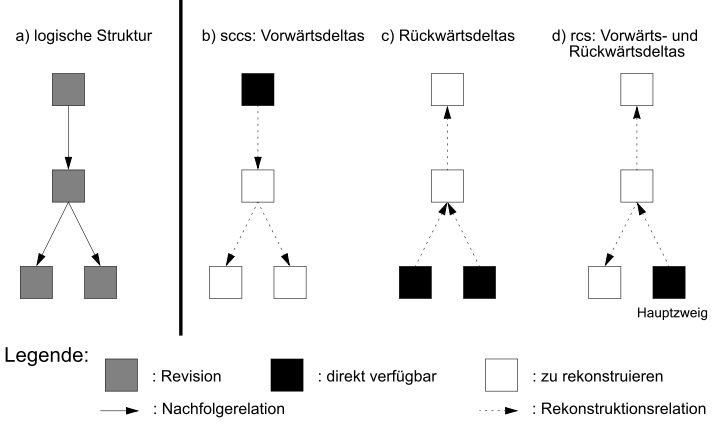
\includegraphics[width=0.85\textwidth]{2_2_1}
\end{figure}
\subsubsection{Concurrent Version (Management) System CVS}
Zunächst Aufsatz auf RCS (später Reimplementierung), das Revisionsverwaltung für ganze Directorybäume durchführt und zusätzlich anbietet:
\begin{itemize}
	\item optimistisches Sperrkonzept mit (fast) \textbf{automatischem Verschmelzen} (merge) von parallel durchgeführten Änderungen in verschiedenen privaten Arbeitsbereichen
	\begin{itemize}
		\item Dreiwegeverschmelzen mit manueller Konfliktbehebung
	\end{itemize}
	\item \textbf{Revisionsidentifikation} und damit rudimentäres \textbf{Releasemanagement} auch durch frei wählbare Bezeichner
	\begin{itemize}
		\item Auszeichnen zusammengehöriger Revisionen durch symbolische Namen (mit Hilfe sogenannter Tags)
	\end{itemize}
	\item diverse \textbf{Hilfsprogramme} 
	\begin{itemize}
		\item wie z.B. ''cvsann'', das jeder Zeile einer Textdatei die Information voranstellt, wann sie von wem zum letzten Mal geändert wurde
	\end{itemize}
\end{itemize}
\begin{figure}
	\caption{Dreiwegeverschmelzen von (Text-)Dateien: }
	\centering
	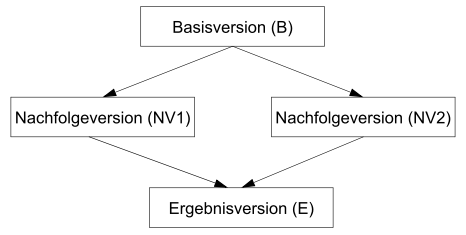
\includegraphics[width=0.5\textwidth]{2_2_2}
\end{figure}
\paragraph{Optimistisches Sperrkonzept mit ''Merge''}
\begin{itemize}
\item Entwickler A macht \textbf{checkout} einer Revision n
\item Entwickler A verändert Revision n lokal zu n1
\item Entwickler B macht \textbf{checkout} derselben Revision n
\item Entwickler B verändert Revision n lokal zu n2
\item Entwickler B macht \textbf{commit} seiner geänderten Revision n2
\item Entwickler A versucht commit seiner geänderten Revision n1
\begin{itemize}
	\item wird mit Fehlermeldung abgebrochen
\end{itemize}
\item Entwickler A macht \textbf{update} seiner geänderten Revision n1 
\begin{itemize}
	\item automatisches merge von n1 und n2 mit Basis n führt zu n'
\end{itemize}
\item Entwickler A löst Verschmelzungskonflikte manuell auf und erzeugt n''
\item Entwickler A macht \textbf{commit} von Revision n'' (inklusive Änderungen von B)
\end{itemize}
\paragraph{Synchronisierung mit Watch/Edit/Unedit:}
In manchen Fällen will man wegen größerer Umbauten eine Datei(-Revision) ''ungestört'' bearbeiten, also zumindest eine Meldung erhalten, wenn andere Entwickler dieselbe Datei bearbeiten (um sie zu warnen):
\begin{itemize}
	\item \textbf{watch on} schaltet das Beobachten einer Datei ein; beim checkout wird die gewünschte Revision der Datei nur mit Leserecht lokal zur Verfügung gestellt
	\item \textbf{watch off} ist das Gegenstück zu watch on
	\item \textbf{watch add} nimmt Entwickler in Beobachtungsliste für Datei auf, für die er vorher ein checkout gemacht hat (Änderungen an Revisionen der Datei werden per Email allen Entwicklern auf Beobachtungsliste gemeldet)
	\item \textbf{watch remove} entfernt Entwickler von Beobachtungsliste für Datei
	\item \textbf{edit} verschafft Entwickler Schreibrecht auf lokal verfügbarer Revision einer Datei und meldet das anderen „interessierten“ Entwicklern (enthält watch add)
	\item \textbf{unedit} nimmt Schreibrecht zurück und meldet das (enthält watch remove)
\end{itemize}
\paragraph{Identifikation gewünschter Revisionen - Zusammenfassung:}
\begin{enumerate}
	\item Verwendung von \textbf{Revisionsnummern} (Identifikatoren): jede Revision einer Datei erhält eine eigene eindeutige Nummer, über die sie angesprochen wird; Nummer werden nach einem bestimmten Schema erzeugt.
	\item Verwendung von \textbf{Attributen} (Tags): Revisionen werden durch Attribute und deren Werte indirekt identifiziert; Beispiele sind:
	\begin{itemize}
		\item Kunde (für den Revision erstellt wurde)
		\item Entwicklungssprache (Java, C,..)
		\item Entwicklungsstatus (in Bearbeitung, getestet, freigegeben,..)
	\end{itemize}
	\item Verwendung von \textbf{Zeitstempeln} (Spezialfall der attributbasierten Identifikation): für jede Revision ist der Zeitpunkt ihrer Fertigstellung (commit) bekannt; deshalb können Revisionen über den Zeitraum ihrer Erstellung (jüngste Revision, vor Mai 2003, etc.) identifiziert werden.
\end{enumerate}
\paragraph{Offene Probleme mit Deltaspeicherung und Verschmelzen}
\begin{itemize}
	\item Berechnung von \textbf{Deltas} funktioniert hervorragend für Textdateien (mit Zeilenenden als ''Synchronisationspunkte'' für Vergleich)
	\item Berechnung minimaler Deltas von Binärdateien ist wesentlich schwieriger 
	\item Textverarbeitungsprogramme wie Word oder CASE-Tools besitzen deshalb eigene Algorithmen zur Berechnung (und Anzeige) von Deltas
	\item Verschmelzung von Textdateien funktioniert meist gut (kann aber zu tückischen Inkonsistenzen führen)
	\item Verschmelzung von Binärdateien oder Grafiken/Diagrammen ist im allgemeinen nicht möglich
	\item Programme wie Word oder CASE-Tools besitzen deshalb eigene Verschmelzungsfunktionen
\end{itemize}
\paragraph{Verbleibende Mängel von CVS}
\begin{itemize}
	\item zugeschnitten auf Textdateien bei (Deltaberechnung und Verschmelzen)
	\item keine Versionierung von Verzeichnisstrukturen (Directories)
	\item nicht integriert mit ''Build-'' und ''Changemanagement''
	\item keine gute Unterstützung für geographisch verteilte Software-Entwicklung
	Inhalt...
\end{itemize}
Aber:
\begin{itemize}
	\item Als ''Open Software'' ohne Anschaffungskosten erhältlich
	\item Administrationsaufwand hält sich in Grenzen
	\item für Build- und Changemanagement gibt es ergänzende Punkte
\end{itemize}
\subsubsection{CVS-Nachfolger Subversion (SVN}
\begin{itemize}
	\item immer ganze Dateibäume werden durch commit versioniert (inklusive Erzeugen, Löschen, Kopieren und Umbenennen von Dateien und Unterverzeichnissen)
	\item commit ganzer Verzeichnisse ist eine atomare Aktion (auch bei Server-Abstürzen, Netzwerkzusammenbrüchen, ... ), die ganz oder gar nicht erfolgt
	\item Metadaten (Dateiattribute, Tags) werden als versionierte Objekte unterstützt
	\item Deltaberechnung funktioniert für beliebige Dateien (auch Binärdateien); Verschmelzungsoperationen sind aber weiterhin eher auf Textdateien zugeschnitten
	\item geographisch verteilte Softwareentwicklung wird besser unterstützt; Dateibäume und Dateien werden durch URLs identifiziert, Datenaustausch kann über http-Protokoll erfolgen
	\item Ungeöhnliche, aber einfache bzw. effiziente Behandlung von mehreren Entwicklungszweigen sowie von Systemrevisionen mit bestimmten Eigenschaften (Tags) als ''lazy copies'' (keine echten Kopien, sondern nur neue Verweise/Links)
\end{itemize}
\paragraph{Einsatz von merge in SVN}
svn merge -r <snapshopt1>:<snapshot2> <source> [<wcpath>]
\\
Dieses Kommando berechnet
\begin{itemize}
	\item  alle Unterschiede zwischen <snapshot1> und <snapshot2> (als Vorwärts- bzw. Rückwärtsdelta) des Verzeichnisses <source> mit allen Unterverzeichnissen und Dateien
	\item und wendet die Änderungen auf die Dateien im aktuellen Workspace-Verzeichnis (ggf. angegeben durch <wcpath> = Working Copy Path) an
	\item geändert werden dabei einzelne Dateien und ganze (Unter-)Verzeichnisse
\end{itemize}
\paragraph{Variante des merge-Kommandos}
svn merge <src1>[@<snapshot1>]<src2>[@<snapshot2>][<wcpath>]
\\
Dieses Kommando wendet das Delta zweier verschiedener Dateien oder Unterverzeichnisse vorgegebener Revisionen (durch Snapshot-Nummer) auf den aktuellen Workspace an. Wird keine Revision angegeben, so wird jeweils die neueste Revision (Head) verwendet.
\paragraph{Delta-Speicherung in svn:}
\begin{itemize}
	\item BDB-Lösung (basierend auf Berkely Database; älterer Ansatz);
	\begin{itemize}
		\item alles wird in einer Datenbank gespeichert
		\item Revisionen werden als Rückwärts-Deltas zu Nachfolgern gespeichert (ähnlich wie bei RCS)
	\end{itemize}
	\item FSFS-Lösung (File System on top of File System; neuer Ansatz)
	\begin{itemize}
		\item Versioniertes Dateisystem, das auf einem ''normalen'' Dateisystem aufsetzt
		\item Revisionen werden als Vorwärts-Deltas zu direkten oder indirekten Vorgängern gespeichert
		\item Die erste Revision ist eine leere Datei
		\item sogenannter ''Skip-List''-Ansatz reduziert Rekonstruktionszeiten durch geschickte Auswahl der Vorgänger
	\end{itemize}
\end{itemize}
\paragraph{Vorwärts-Delta-Speicherung mit ''Skip-List''- Ansatz in SVN}
Subversion kehrt für die effiziente Speicherung von Revisionen zum ''Vorwärtsdelta''-Ansatz von SCCS zurück, benötigt aber bei einer Liste von n aufeinander folgenden Revisionen nur log n Rekonstruktionsschrite. Das funktioniert wie folgt mit $r_{i} = i-te $ Revision und $d_{i,j} = Delta$ von $r_{i}$ nach $r_{j}$:
\begin{itemize}
	\item Revision $r_{0}$ ist immer leere Datei.
	\item Revision $r_{1}$ wird durch Anwendung des Deltas $d_{0,1}$ auf $r_{0}$ erzeugt.
	\item Revision $r_{2}$ wird durch Anwendung des Deltas $d_{0,2} = d_{0,1} und d_{0,2}$ auf $r_{0}$ erzeugt.
	\item Revision $r_{3}$ wird durch Anwendung des Deltas $d_{2,3}$ auf $r_{2}$ erzeugt, das seinerseits wiederum durch ... erzeugt wird.
\end{itemize}
\textbf{Achtung:} Die Konkatenation $d_{i,j} und d_{j,k}$ zweier Deltas ist oft \textbf{deutlich kürzer} als die Summe der Länge der beiden konkatenierten Deltas (aufgrund sich aufhebender Editierschritte).
\\
\\
Für die Berechnung des direkten Vorgängers $r'$ zu einer Revision $r$ wird das letzte 1-Bit der Binärdarstellung von r auf ''0'' gesetzt; die sich daraus ergebende Zahl legt r' fest, auf das Delta $d_{r,r'}$ zur Konstruktion von r angwendet wird (rekursiver Prozess!).
\subsubsection{Geschichte verteilter Versionierungs-Systeme}
\textbf{VCS} = Version Control System
\\
\textbf{DVCS} = Distributed Version Control System
\begin{figure}[h]
	\caption{Geschichte verteilter Versionierungs-Systeme}
	\centering
	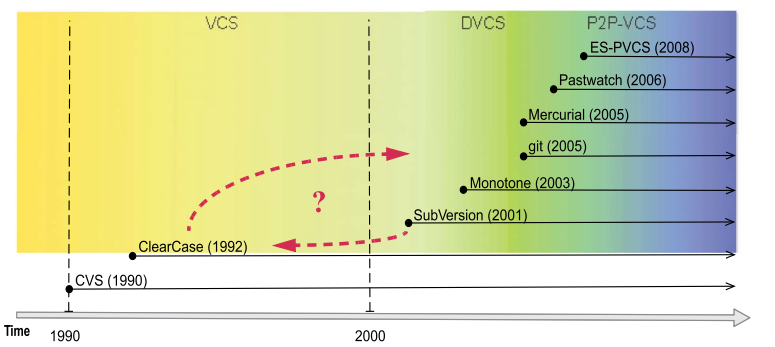
\includegraphics[width=0.8\textwidth]{2_2_3}
\end{figure}
\paragraph{Anmerkung zu ''Urahn'' ClearCase:}
Das System ist ein Grenzfall zwischen VCS und DVCS. Es handelt sich zwar um kein reines CSS mehr, aber die Verteilung auf mehrere Server und deren Kooperation hat doch noch sehr zentralistischen Charakter im Gegensatz zu den ''reinen'' DVCS, die auf dem Rechner eines jeden Entwicklers eine eigene Instanz laufen haben.
\subsubsection{''Echt'' verteilte Versionierungs-Systeme:}
\textbf{Jeder} Benutzer hat sein eigenes vollständiges Repository (statt globale Repositories für Teilgruppen von Entwicklern wie bei ClearCase).
\begin{itemize}
	\item \textbf{Push:} Revisionen zu anderen Repositories aktiv propagieren
	\item \textbf{Pull:} Revisionen von anderen Repositories aktiv holen
\end{itemize}
\paragraph{Prinzipien ''echt'' verteilter Versionierungs-Systeme wie ''git'':}
\begin{itemize}
	\item Jeder Entwickler hat eigenes lokales Versionierungs-Repository mit Snapshots wie bei SVN (Subversion) zusätzlich zu  üblichen Arbeitskopien von Dateien
	\item Check-Out, Commit, ... arbeiten erst mal nur auf eigenen lokalem Repository
	\item Austausch zwischen Repositories erfolgt mit Push und Pull (zwischen bekannten Personen/Rechnern) via Email oder ssh oder ... 
	\item Bei Push/Pull werden parallele Revisionen angelegt, die dann mit ''merge'' zusammengeführt werden (müssen) 
\end{itemize}
\paragraph{Bewertung:}
\begin{itemize}
	\item \textbf{+} Entwickler können auch ''offline'' mit eigenem Repository arbeiten
	\item \textbf{+} Änderungen können zu selbst gewähtem Zeitpunkt integriert werden (merge)
	\item \textbf{-} Nach Platten-Crash ist lokales Repository weg
	\item \textbf{-} Hoher Aufwand für Verteilung von Änderungen an andere Entwickler (merge)
\end{itemize}
\subsubsection{Verteilte ''Peer-to-Peer''-Versionierungs-Systeme:}
\begin{itemize}
	\item \textbf{Virtuell} existiert ein \textbf{gemeinsames globales Repository} für alle Entwickler
	\item Es gibt dennoch keinen ausgewählten zentralen Server
	\item Tatsächlich besitzt jeder Peer ein eigenes Repository (mit allen Dateien oder ausgewählter Menge von Revisionen)
	\item Das P2P-Versionierungs-System ist ''immun'' gegen Ausscheiden einzelner Peers (Revisionen werden auf mehreren Peers gehalten)
	\item Bei \textbf{Netzpartitionierungen} (Spezialfall: einzelner Entwickler arbeitet ''offline'' wird je Partition ein eigener Branch angelegt
	\item Schließen sich Partitionen wieder zusammen, dann werden Branches wieder verschmolzen (im allgemeinen mit Entwicklerhilfe)
\end{itemize}
\paragraph{Fazit:}
P2P-Versionierungssysteme sollen die Vorteile von VCS und DVCS vereinen!
\subsection{Variantenmanagement (Software-Produktlinien}
Das Variantenmanagement befasst sich mit der Verwaltung nebeneinander existierender Versionen eines Dokuments, die jeweils eine zeitliche Entwicklungsgeschichte besitzen
\paragraph{Software-Produktlinien-Entwicklung = ''Variantenmanagement im Großen''}
Eine \textbf{Software-Produkt-Linie} (SPL) ist eine Menge ''verwandter'' Softwareysteme
\begin{itemize}
	\item für eine bestimmte \textbf{Anwedungsdomäne}
	\item die auf Basis einer gemeinsamen \textbf{Plattform} (Rahmenwerk)
\end{itemize}
entwickelt werden. Die Plattform enthält alle SW-Artefakte, die für alle Instanzen der Produktlinie gleich sind. Damit ist die Software-Produktlinien-Entwicklung (SPLE = Software Product Line Engineering) eine logische Verallgemeinerung des Variantenmanagements eines Softwaresystems.
\\
Man unterscheidet beim SPLE zwischen
\begin{itemize}
	\item der \textbf{Domänenentwicklung} (Domain Engineering) der gemeinsamen Plattform (development \textbf{for} reuse)
	\item der \textbf{Anwendungsentwicklung} (Application Engineering) von SPL-Instanzen (development \textbf{with} reuse)
\end{itemize}
\begin{figure}[h]
	\centering
	\caption{Domänen- und Anwendungsentwicklung}
	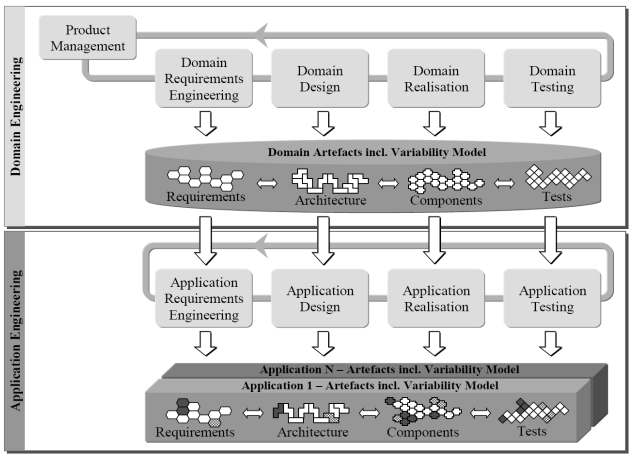
\includegraphics[width=0.6\textwidth]{2_3_1}
\end{figure}
\paragraph{Variabilitätsmodell (Feature-Modell) einer SPL:}
So genannte Variabilitäts- oder Fature-Modelle beschreiben alle möglichen Eigenschaften einer Software-Produktlinie und zulässige Kombinationen (Konfigurationen, Varianten, Instanzen) dieser Produktlinie. 
\\
\\
Eine Vielzahl von Notationen und Werkzeugen unterstützen die Erstellung solcher Modelle durch
\begin{itemize}
	\item Festlegung aller auswählbaren Eigenschaften/Merkmale = \textbf{Features} der Instanzen der Produktlinie (vor allem die optionalen/alternativen Eigenschaften)
	\item \textbf{hierarchische Zerlegung} von Merkmalen in Untermerkmale
	\item Festlegung von \textbf{Auswahl-Optionen} der Art eins-aus-n, m-aus-n,..
	\item Definition von \textbf{Abhängigkeiten} und Ausschlusskriterien einzelner Merkmale in ganz verschiedenen Teilhierarchien
\end{itemize}
\paragraph{Werkzeugunterstützung für SPL-Entwicklung:}
\begin{itemize}
	\item (grafische) Erstellung von Variabilitätsmodellen
	\item Unterstützung bei der Auswahl erlaubter Merkmalkombinationen
	\item Erzeugung von Produktinstanzen (Implementierungen) für bestimmte Merkmalkombinationen
	\item Unterstützung beim systematischen Test von SPLs
\end{itemize}
\paragraph{Grafische Notation von FeatureIDE:}
\begin{itemize}
	\item \textbf{Mandatory:} ist immer ausgewählt (falls Elternfeature gewählt)
	\item \textbf{Optional:} kann beliebig an- oder abgewählt werden (falls Elternfeature gewählt)
	\item \textbf{Or:} mindestens ein Feature ist auszuwählen (falls Elternfeature gewählt)
	\item \textbf{Alternative:} genau eins muss ausgewählt werden
	\item \textbf{x -> y:} wenn X gewählt wird, dann auch Y
\end{itemize}
\begin{figure}[h]
	\centering
	\caption{Grafische Notation von FeatureIDE}
	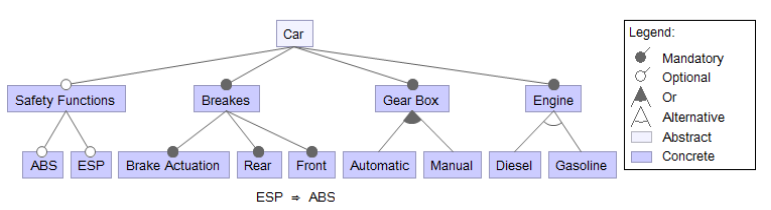
\includegraphics[width=0.85\textwidth]{2_3_2}
\end{figure}
\subsubsection{Variantenmanagement für Quelltextdateien:}
Hierfür gibt es kaum eigene Unterstützung. Im wesentlichen bleiben folgende Möglichkeiten zur Verwaltung verschiedener Varianten eines Dokuments:
\begin{itemize}
	\item Mit Hilfe der \textbf{Versionsverwaltung} wird je Variante ein eigener Entwicklungszweig gepflegt (mit entsprechendem Tag). Änderungen von einem Zweig werden mit Hilfe der Dreiwegeverschmelzung in andere Zweige propagiert.
	\item  Die verschiedenen Varianten werden alle in einer Datei gespeichert; durch \textbf{Bedingungsmakros} ( \#ifdef Unix ... ) werden die für eine Variante benötigten Quelltextteile ein- und ausgeblendet (siehe pure::variants)
	\item Die verschiedenen Varianten einer Klassenimplementierung werden in Unterklassen ausgelagert (Einsatz von \textbf{Vererbung})
	\item Benötigte Varianten werden (aus einer domänenspezifischen Beschreibung) \textbf{generiert} (mit Quelltexttransformationen, aspektorientierter Programmierung, ... )
	\item \textbf{Achtung}: Auswahl/Konfiguration/Transformation benötigter Quelltextdateien durch das Build-Management
\end{itemize}
\subsection{Releasemanagement}
Ein Release ist eine an Kunden ausgelieferte Konfiguration eines (Software-)Systems bestehend aus ausführbaren Programmen, Bibliotheken, Dokumentation, Quelltexte, Installationsskripte, ... . 
\\
\\
Das Releasemangement dokumentiert ausgelieferte Konfigurationen und stellt deren Rekonstruierbarkeit sicher.
\subsubsection{Aufgaben des Releasemanagement}
\begin{itemize}
	\item Festlegung der (zusätzlichen) Funktionalität eines neuen Releases
	\item Festlegung des Zeitpunktes der Freigabe eines neuen Releases 
	\item  Erstellung und Verbreitung eines Releases (siehe auch Buildmanagement)
	\item  Dokumentation des Releases:
	\begin{itemize}
		\item welche Revisionen welcher Dateien sind Bestandteil des Releases
		\item welche Compilerversion wurde verwendet
		\item Betriebssystemversionen auf Entwicklungs- und Zielplattform
	\end{itemize}
\end{itemize}
\subsubsection{Planungsprozess für neue Releases:}
\begin{enumerate}
	\item Vorbedingungen für neues Release werden überprüft:
	\begin{itemize}
		\item viel Zeit vergangen (neues Release aus Publicity-Gründen)
		\item viele Fehler behoben (neues Release mit allen ''Patches'')
		\item viele neue Funktionen hinzugefügt
	\end{itemize}
	\item Weiterentwicklung wird eingefroren (freeze):
	\begin{itemize}
		\item \textbf{Feature Freeze} (Soft Freeze): nur noch Fehlerkorrekturen und kleine Verbesserungen erlaubt (nur vermutlich nicht destabilisierende Änderungen)
		\item  \textbf{Code Freeze} (Hard Freeze): nur noch absolut notwendige Änderungen, selbst ``gefährliche'' Fehlerkorrekturen werden verboten
	\end{itemize}
	\item Letzte Fehlerkorrekturen und umfangreiche Qualitätssicherungsmaßnahmen (Tests) werden durchgeführt
	\item Release wird freigegeben und weiterverbreitet:
	\begin{itemize}
		\item Weiterentwicklung (neuer Releases) wird wieder aufgenommen
		\item freigegebenes Release muss parallel dazu gepflegt werden
	\end{itemize}
\end{enumerate}
\paragraph{Standardlösung für parallele Pflege und Weiterentwicklung:}
\begin{itemize}
	\item für Weiterentwicklung des nächsten Releases und Wartung des gerade freigegebenen Releases werden unterschiedliche Revisionszweige verwendet
	\item alle auf dem Wartungszweig liegenden Revisionen erhalten den Namen des Releases (Versionsnummer) als Tag
\end{itemize}
\paragraph{Strategien für die Vergabe von Versions- und Revisionsnummern:}
\begin{itemize}
	\item Software-Releases erhalten üblicherweise zweistellige \textbf{Versionsnummern}
	\item die erste Stelle wird erhöht, wenn sich die Funktionalität signifikant ändert
	\item die zweite Stelle wird für kleinere Verbesserungen erhöht
	\item oft wird erwartet, dass  x.2, x.4, ...  stabiler als  x.1, x.3, ... sind
	\item die (in cvs vierstelligen) internen \textbf{Revisionsnummern} eines KM-Systems müssen mit den extern sichtbaren Versionsnummern nichts zu tun haben
	\item in den vorigen Beispielen galt aber: \\
	Versionsnummer = ersten beiden Stellen der Revisionsnummer
	\item oft werden jedoch die ersten beiden Stellen der Revisionsnummern 
	(in cvs) nicht verwendet und bleiben auf ``1.1'' gesetzt
\end{itemize}
\subsection{Buildmanagement}
Das Buildmanagement (Software Manufacturing) automatisiert den Erzeugungsprozess von Programmen (Software Releases).
\subsubsection{Werkzeuge für das Build-Management}
\begin{itemize}
	\item Das Werkzeug \textbf{''make''} (im folgenden im Detail präsentiert): 
	\begin{itemize}
		\item deklarativer, regelbasierter Ansatz
		\item es werden Abhängigkeiten zwischen Entwicklungsartefakten definiert (mit zusätzlichen Kommandos zur Erzeugung abgeleiteter Artefakte)
		\item unabhängig v. Entwicklungsprozess, Programmiersprachen, Werkzeugen
	\end{itemize}
	\item Das Werkzeug \textbf{''Ant''} (make-Nachfolger im Java-Umfeld):
	\begin{itemize}
		\item gemischt deklarativer bzw. imperativer Ansatz
		\item es werden Abhängigkeiten zwischen Aufgaben (Tasks) definiert
		\item Tasks können mit Kontrollstrukturen ''ausprogrammiert'' werden
		\item verwendet XML-Syntax für Konfigurationsdateien
		\item in Java und vor allem für Java-Projekte entwickelt
		\item aber: unabhängig von Entwicklungsprozess, Projektstruktur, ...
	\end{itemize}
	\item Das Werkzeug \textbf{''Maven''}: 
	\begin{itemize}
		\item deklarativer Ansatz mit relativ einfachen Konfigurationsdateien
		\item macht viele Annahmen über Entwicklungsprozess, Projektstruktur, ...
		\item  keine frei definierbaren Regeln für bestimmte Sprachen, Werkzeuge sondern stattdessen Plugins
		\item Fokus liegt auf der Unterstützung von Java-Projekten
		\item holt sich Plugins, Libraries, ... aus zentralen Repositories
		\item oft kombiniert mit ''Nexus'' für Einrichten lokaler (Cache-)Repositories
	\end{itemize}
	\item Das Werkzeug \textbf{''Jenkins''} (früher: ''Hudson''):
	\begin{itemize}
		\item ergänzt Build-Werkzeuge wie Ant und Maven
		\item unterstützt die kontinuierliche Integration/Auslieferung von Produkten
		\item automatische Integration von Build-, Test-, Reporting-Werkzeugen
	\end{itemize}
\end{itemize}
\subsubsection{Das Programm ''make'' zur Automatisierung von Build-Vorgängen:}
\begin{itemize}
	\item \textbf{make} wurde in den 70er Jahren ''nebenbei'' von Stuart F. Feldman für die Erzeugung von Programmen unter Unix programmiert
	\item Varianten von make gibt es heute auf allen Betriebssystemplattformen (oft integriert in oder spezialisiert auf Compiler einer Programmiersprache) 
	\item make werden durch ein sogenanntes \textbf{makefile} Erzeugungsabhängigkeiten zwischen Dateien mitgeteilt
	\item make benutzt \textbf{Zeitmarken} um festzustellen, ob eine Datei noch aktuell ist (Zeitmarke jünger als die Zeitmarken der Dateien, von denen sie abhängt)
\end{itemize}
\paragraph{Erläuterungen der seltsamen Sonderzeichen-Makros:}
\begin{itemize}
	\item \textbf{\$@} bezeichnet immer das Ziel einer Regel
	\item \textbf{\$*} bezeichnet immer das Ziel einer Regel ohne Suffix
	\item \textbf{\$\^} bezeichnet alle Objekte einer Regel rechts vom '':''
	\item \textbf{\$?} bezeichnet alle Objekte einer Regel rechts vom '':'', die neuer als das Ziel sind
	\item \textbf{\$<} bezeichnet das erste Objekte rechts vom '':''
\end{itemize}
\paragraph{Muster-Suche und Substitutionen in make:}
Oft benötigt man auf der rechten Seite einer Regel oder in der Kommandozeile alle Dateinamen (im aktuellen Verzeichnis), die einen bestimmten \textbf{Namensmuster} entsprechen (also etwa mit einem bestimmten Suffix enden). \\
\$(wildcard Muster) \\
liefert bzw. \textbf{sucht} alle Dateien im aktuellen Verzeichnis, die dem angegebenen Muster entsprechen. Das Muster kann beispielsweise folgende Form haben: \\
\$(wildcard*.c) \\
liefert alle Dateien zurück, die das Suffix ''.c'' besitzen (der ''*'' matcht alles). 
\\
\\
Will man in einer Liste von Dateinamen (durch Leerzeichen getrennte Strings) einen Teilstring durch einen anderen Teilstring \textbf{ersetzen} (substituieren) verwendet man: \\
\$(patsubst Suchmuster, Ersatzstring, Liste von Wörtern) \\
Folgender Ausdruck ersetzt alle ''.c''-Suffixe durch ''.o''-Suffixe: \\
\$(patsubst\%.c, \%.0, Liste von Wörtern) \\
Das Zeichen ''\%'' bezeichnet den gleichbleibenden Teil bei der Ersetzung.

\paragraph{Muster-Regeln in make:}
Manchmal will man Regeln schreiben, die alle Dateien mit einem bestimmten Präfix oder Suffix aus einer anderen Datei mit unterschiedlichem =Präfix oder Suffix aber ansonsten gleichem Namen errechnen. So wird z.B. jede c-Datei in eine o-Datei ansonsten gleichen Namens übersetzt. Die Muster-Regel ist für die Definition solcher Abhängigkeiten geeignet: \\
prefix1\%suffix1 : prefix1\%.suffix2 ...

\paragraph{Bewertung des Buildmanagements mit make:}
\begin{itemize}
	\item nur ein Bruchteil der Funktionen von make wurde vorgestellt
	\item ursprüngliches make führt Erzeugungsprozesse sequentiell aus
	\begin{itemize}
		\item GNU make kann Arbeit auf mehrere Rechner verteilen und parallel durchführbare Erzeugungsschritte gleichzeitig starten
	\end{itemize}
	\item Steuerung durch Zeitmarken ist sehr ''grob'':
	\begin{itemize}
		\item \textbf{zu häufiges neu generieren}: irrelevante Änderungen (wie Ändern von Kommentaren für Übersetzung) werden nicht erkannt 
		\item \textbf{zu seltenes neu generieren}: Änderung von Übersetzerversionen, Übersetzungsoptionen etc. werden nicht erkannt
	\end{itemize}
	\item kaum Verzahnung mit Versionsverwaltung:
	\begin{itemize}
		\item make wird in aller Regel auf eigenem Repository durchgeführt
		\item erzeugte/abgeleitete Objekte werden also immer privat gehalten
	\end{itemize}
	\item makefiles selbst müssen manuell aktuell gehalten werden
	\begin{itemize}
		\item programmiersprachenspezifisches makedepend erzeugt makefiles
	\end{itemize}
\end{itemize}

\paragraph{Erzeugung von Makefiles:}
\begin{enumerate}
	\item in jedem Quelltextverzeichnis gibt es ein ''normales'' Makefile, das den Übersetzungsprozess mit make in diesem Verzeichnis steuert
	\item ''normale'' Makefiles werden von makedepend durch Analyse von Quelltextdateien erzeugt (in C werden includes von .h-Dateien gesucht)
	\item ein ''Super''-Makefile sorgt dafür, dass 
	\begin{itemize}
		\item makedepend nach relevanten Quelltextänderungen in den entsprechenden Verzeichnissen aufgerufen wird
		\item in allen ''normalen'' Makefiles dieselben Makrodefinitionen verwendet werden (soweit gewünscht)
		\item geänderte Makefiles oder Makrodefinitionen dazu führen, dass in den betroffenen Verzeichnissen alle abgeleiteten Objekte neu erzeugt werden
	\end{itemize}
\end{enumerate}

\paragraph{Generierung von Makefiles mit GNU Autotools}
Die GNU \textbf{Autotools} sind mehrere Werkzeuge, die aufbauend auf make das Build-Management, also die Erstellung und Installation von Softwarekonfigurationen für verschiedenste Zielplattformen, erleichtern. 
\begin{itemize}
	\item Fokus liegt auf Softwareprojekten, in denen vor allem C, C++ oder Fortran (77) als Programmiersprachen eingesetzt werden
	\item die Werkzeuge eignen sich nicht (kaum) für Java-Projekte oder SW-Entwicklung im Windows-Umfeld
	\item \textbf{Automake} unterstützt Generierung „guter“ makefiles aus deutlich kompakteren Konfigurationsdateien (die von allen populären make-Varianten ausführbar sind)
	\item \textbf{Autoconf} unterstützt Konfigurationsprozess von Software durch Generierung von config.h-Skeletten, Konfigurationsskripten, ...  
	\item schließlich gibt es noch \textbf{Libtool}, das Umgang mit Bibliotheken erleichtert
\end{itemize}
\subsubsection{Zusammenfassung und Ratschläge:}
\begin{itemize}
	\item Bereits in kleinsten Projekten ist die Automatisierung von Erzeugungsprozessen (Buildmanagement) ein Muss; in einfachen Fällen die notwendige Unterstützung.
	\item Im Linux/Unix-Umfeld ist ''(GNU) make'' das Standardwerkzeug für die Automatisierung von Erzeugungsprozessen.
	\item In jedem Projekt sollte es genau einen Verantwortlichen für die Pflege von Konfigurationsdateien (Makefiles) und Build-Prozesse geben.
	\item Für Java-Programmentwicklung gibt es mit Ant ein speziell zugeschnittenes moderneres ''Build-Tool''
	\item Noch ''moderner'' sind Maven und Jenkins für ''Continuous Integration'', also die automatisierte, permanente Erzeugung von Software-Releases.
	\item Nicht generierte (Anteile von) Konfigurationsdateien müssen selbst unbedingt der Versionsverwaltung unterworfen werden.
\end{itemize}
\subsection{Änderungsmanagement}
Ein festgelegter Änderungsmanagementprozess sorgt dafür, dass Wünsche für Änderungen an einem Softwaresystem protokolliert, priorisiert und kosteneffektiv realisiert werden.

\subsubsection{Änderungsmanagement frei nach [Li02]}
Ausfüllen eines Änderungsantragsformulars; \\
Analyse des Änderungsantrags; \\
\textbf{if} Änderung notwendig (und noch nicht beantragt \textbf{then} \\
Bewertung wie Änderung zu implementieren ist; \\
Einschätzung der Änderungskosten; \\
Einreichen der Änderung bei Kommission; \\
\textbf{if} Änderung akzeptiert \textbf{then} \\
Durchführen der Änderung für Release... \\
\textbf{else} \\
Änderungsantrag ablehnen \\
\textbf{else} \\
Änderungsantrag ablehnen

\subsubsection{Änderungsmanagement frei nach [Wh00]}
\begin{enumerate}
	\item ein Änderungswunsch (feature request) oder eine Fehlermeldung (bug report) wird eingereicht (Status \textbf{submitted})
	\item ein eingereichter Änderungswunsch wird evaluiert und dabei
	\begin{itemize}
		\item entweder abgelehnt (Status \textbf{rejected})
		\item oder als Duplikat erkannt (Status \textbf{duplicate})
		\item oder mit Kategorie und Priorität versehen (Status \textbf{accepted})
	\end{itemize}
	\item ein akzeptierter Änderungswunsch wird von dem für seine Kategorie Zuständigen
	\begin{itemize}
		\item für ein bestimmtes Release zur Bearbeitung freigegeben (Status \textbf{assigned})
		\item oder vorerst aufgeschoben (Status \textbf{postponed})
	\end{itemize}
	\item ein zugewiesener Änderungswunsch wird von dem zuständigen Bearbeiter in Angriff genommen (Status \textbf{opened})
	\item irgendwann ist die Bearbeitung eines Änderungswunsches beendet und die Änderung wird zur Prüfung freigegeben (Status \textbf{released})
	\item erfüllt die durchgeführte Änderung den Änderungswunsch, so wird schließlich der Änderungswunsch geschlossen (Status \textbf{closed})
\end{enumerate}

\paragraph{Funktionalität von Änderungsmanagement-Werkzeugen:}
\begin{itemize}
	\item Änderungswünsche können über Browserschnittstelle übermittelt werden
	\item Änderungswünsche werden in Datenbank verwaltet
	\item Betroffene werden vom Statuswechsel eines Änderungswunsches benachrichtigt
	\item Integration mit Projektmanagement und KM-Management
	\item Trendanalyse und Statistiken als Grafiken (Anzahl neuer Fehlermeldungen, ... )
\end{itemize}

\paragraph{Werkzeuge für das Änderungsmanagement:}
\begin{itemize}
	\item ''Open Software''-Produkt \textbf{Sourceforge} (GForge), das cvs/svn/git/... mit Änderungsmanagementdiensten kombiniert
	\item Neuere Alternativen zu Sourceforge: GitHub, GitLab, BitBucket, ... 
	\item ''Open Software''-Produkt \textbf{Bugzilla} für reines Änderungsmanagement 
	\item flexibles Projektmanagement-Werkzeug \textbf{Redmine} mit Aufgabenverwaltung, Versionsverwaltung (cvs/svn/git/... ) etc.
\end{itemize}

\subsection{Zusammenfassung}
Mit einem für die jeweilige Projektgröße sinnvollen KM-Management steht und fällt die Qualität eines Softwareentwicklungsprozesses, insbesondere nach der Fertigstellung des ersten Softwarereleases. 
\paragraph{Meine Ratschläge für das KM-Management:}
\begin{itemize}
	\item besteht ihr System aus mehr als einer Handvoll Dateien, so sollte ein \textbf{Buildmanagementsystem} wie make/Ant/Maven verwendet werden
	\item haben sie Entwicklungszeit von mehr als ein paar Tagen oder mehr als einem Entwickler, so ist ein \textbf{Versionsmanagementsystem} wie svn oder git ein Muss
	\item haben sie mehr als einen Anwender oder mehr als ein Release der Software, so ist ein \textbf{Changemanagementsystem} wie in Bugzilla/Redmine einzusetzen
	\item Werkzeuge wie Sourceforge, GitHub, GitLab, ... , die Versionsmanagement mit Bugtracking, Wiki-Dokumentation etc. kombinieren, immer einsetzen! Alles weitere hängt von Projektgröße und Kontext ab.
\end{itemize}



